\subsection{\textbf{WP-01}: \gls{USDF} Infrastructure}
\label{sect:wp01}
The main deliverable is a computing infrastructure capable of supporting
the Rubin Observatory Data Production operations. The organizational structure of Rubin Observatory is presented in detail in the Operations Plan document  \citedsp{LDO-31}.

\tabref{tab:storageFloorOps}  gives the estimated high level storage needs for operations.
\tabref{tab:computeSizingOps} gives the estimated high level compute needs for ops.
More details are provided in \appref{sec:sizeinputs} and a graphical
representation of storage needs is given in \figref{fig:storage}.


These are of course estimates, algorithms may be less (or more) efficient and sizes may prove to be slightly off. The USDF should monitor the actual situation with Rubin Observatory and decide how to address any
situation which arises including raising it to the funding agencies if appropriate. Furthermore, the technical requirements in these documents capture key platforms and services that will be delivered by the Construction Project to Operations. They are not an exhaustive list, and as big data science is a rapidly evolving field, may evolve or be superseded during Operations.

\begin{figure}
\begin{center}
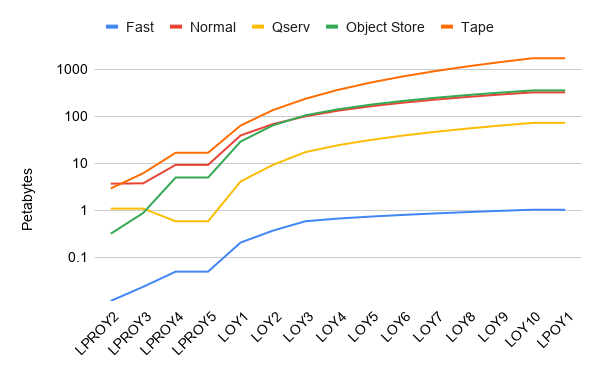
\includegraphics[width=0.8\textwidth]{figs/storage}
\end{center}
\caption{Evolution of {\bf cumulative} storage needs for Rubin Observatory. Details are given in the appendix. This plot shows the total storage needed at the \gls{USDF} of different types. Storage at other data facilities, including the Chilean data access center, are not included here. The \gls{USDF} is responsible for the last two years of pre operations (LPROY4-5) which are transition to \gls{USDF}, the survey years (LOY1-10), and the post operations years (only the first year of two is shown).\label{fig:storage}}
\end{figure}

There is an existing agreement with IN2P3 \citedsp{Agreement-51} to provision and execute 50\% of the total Data Release Production; the \gls{USDF} awardee will need to work with IN2P3 to enable this production.
It is incumbent upon the \gls{USDF}to develop and deploy systems for effectively managing split-site data processing.

Another facility may yet provide a further 25\% of processing power which would also have to be integrated in the model. If that happens, then the corresponding scope would be removed from the \gls{USDF}. For purposes of the \gls{FOA}, it can be assumed the \gls{USDF} will do 50\% of the Data Release Production.

The price of disk and tape media purchases over time have a profound effect on the \gls{USDF} budget over 10 years.
The FOA proposal should explicitly state the assumed pricing factors over the life of the survey for annual hardware purchases. It is assumed that the cost of media will decrease over time, and the annual decrements should be called out in the proposal (net of annual consumer inflation).


\tiny \begin{longtable} { |p{0.22\textwidth}  |r  |r  |r  |r  |r  |r  |r  |r  |r  |r  |r  |r |} 
\caption{On floor LDF storage estimates during Operations
 \label{tab:storageFloorOps}}\\ 
\hline 
\textbf{LDF Storage (on the floor)}&\textbf{unit}&\textbf{LOY1}&\textbf{LOY2}&\textbf{LOY3}&\textbf{LOY4}&\textbf{LOY5}&\textbf{LOY6}&\textbf{LOY7}&\textbf{LOY8}&\textbf{LOY9}&\textbf{LOY10} \\ \hline
{APDB}&{TB}&{24}&{24}&{24}&{24}&{24}&{24}&{24}&{24}&{24}&{24} \\ \hline
{Qserv Czar/ Object}&{TB}&{182}&{347}&{562}&{643}&{711}&{774}&{835}&{894}&{951}&{1006} \\ \hline
\textbf{Total Fast}&\textbf{TB}&\textbf{206}&\textbf{371}&\textbf{586}&\textbf{667}&\textbf{735}&\textbf{798}&\textbf{859}&\textbf{918}&\textbf{974}&\textbf{1029} \\ \hline
{Normal}&{TB}&{38983}&{67976}&{99538}&{131025}&{162321}&{193727}&{225288}&{256991}&{288788}&{320731} \\ \hline
{Qserv Storage}&{TB}&{4094}&{9257}&{17275}&{24144}&{31277}&{38734}&{46555}&{54716}&{63206}&{72017} \\ \hline
{LSSTCam Raw Images}&{TB}&{6982}&{11798}&{16614}&{21430}&{26246}&{31062}&{35878}&{40694}&{45510}&{50326} \\ \hline
{LSSTCam Output Images}&{TB}&{3933}&{10676}&{16857}&{23599}&{30342}&{37084}&{43827}&{50570}&{57312}&{64055} \\ \hline
{LSSTCam Output Coadd Images}&{TB}&{8636}&{16364}&{23182}&{23182}&{23182}&{23182}&{23182}&{23182}&{23182}&{23182} \\ \hline
{LSSTCam Output Parquet}&{TB}&{9302}&{25248}&{47839}&{71758}&{95678}&{119597}&{143516}&{167436}&{191355}&{215275} \\ \hline
{Object Store}&{TB}&{28854}&{64086}&{104491}&{139969}&{175447}&{210925}&{246403}&{281881}&{317359}&{352837} \\ \hline
{LSSTCam Raw Images}&{TB}&{6982}&{11798}&{16614}&{21430}&{26246}&{31062}&{35878}&{40694}&{45510}&{50326} \\ \hline
{All Data Products/ Backup}&{TB}&{47626}&{106967}&{194226}&{309242}&{451681}&{621564}&{818915}&{1043758}&{1296109}&{1575992} \\ \hline
{All Object Store-Only Products}&{TB}&{8636}&{16364}&{24091}&{31818}&{39545}&{47273}&{55000}&{62727}&{70455}&{78182} \\ \hline
{Tape}&{TB}&{63245}&{135129}&{234931}&{362490}&{517473}&{699899}&{909793}&{1147179}&{1412074}&{1704500} \\ \hline
\end{longtable} \normalsize

\tiny \begin{longtable} { |p{0.22\textwidth}  |r  |r  |r  |r  |r  |r  |r  |r  |r  |r  |r  |r |} 
\caption{Compute needs during Operations \label{tab:computeSizingOps}}\\ 
\hline 
\textbf{Data Release Production}&\textbf{units}&\textbf{LOY1}&\textbf{LOY2}&\textbf{LOY3}&\textbf{LOY4}&\textbf{LOY5}&\textbf{LOY6}&\textbf{LOY7}&\textbf{LOY8}&\textbf{LOY9}&\textbf{LOY10} \\ \hline
{LSSTCam visit input size}&{TB}&{1911}&{3822}&{5733}&{7644}&{9556}&{11467}&{13378}&{15289}&{17200}&{19111} \\ \hline
{DRP compute}&{core-hours}&{4.5E+07}&{8.2E+07}&{1.2E+08}&{1.6E+08}&{2.0E+08}&{2.5E+08}&{2.9E+08}&{3.3E+08}&{3.7E+08}&{4.1E+08} \\ \hline
{Alert Production}&{units}&{LOY1}&{LOY2}&{LOY3}&{LOY4}&{LOY5}&{LOY6}&{LOY7}&{LOY8}&{LOY9}&{LOY10} \\ \hline
{AP cores}&{cores}&{1,188}&{1,188}&{1,188}&{1,188}&{1,188}&{1,188}&{1,188}&{1,188}&{1,188}&{1,188} \\ \hline
{US DAC}&{units}&{LOY1}&{LOY2}&{LOY3}&{LOY4}&{LOY5}&{LOY6}&{LOY7}&{LOY8}&{LOY9}&{LOY10} \\ \hline
{LSP cores}&{cores}&{517}&{933}&{1,399}&{1,866}&{2,332}&{2,798}&{3,265}&{3,731}&{4,198}&{4,664} \\ \hline
{Qserv data per node}&{TB/ node}&{43}&{43}&{86}&{86}&{86}&{86}&{173}&{173}&{173}&{173} \\ \hline
{Qserv nodes}&{nodes}&{95}&{216}&{309}&{348}&{364}&{451}&{436}&{408}&{367}&{418} \\ \hline
{LSP cores/ science user}&{cores/ user}&{0.1}&{0.2}&{0.2}&{0.2}&{0.3}&{0.4}&{0.4}&{0.5}&{0.6}&{0.6} \\ \hline
{Chilean DAC}&{units}&{LOY1}&{LOY2}&{LOY3}&{LOY4}&{LOY5}&{LOY6}&{LOY7}&{LOY8}&{LOY9}&{LOY10} \\ \hline
{LSP cores}&{cores}&{103}&{187}&{280}&{373}&{466}&{560}&{653}&{746}&{840}&{933} \\ \hline
{Qserv nodes}&{nodes}&{95}&{216}&{309}&{348}&{364}&{451}&{436}&{408}&{367}&{418} \\ \hline
{Staff LSP}&{units}&{LOY1}&{LOY2}&{LOY3}&{LOY4}&{LOY5}&{LOY6}&{LOY7}&{LOY8}&{LOY9}&{LOY10} \\ \hline
{LSP cores}&{cores}&{52}&{93}&{140}&{187}&{233}&{280}&{326}&{373}&{420}&{466} \\ \hline
\end{longtable} \normalsize



\newreqtype{INFR}
\reqsimp{}{}{}{}{}
{
The cost model for work package \ref{sect:wp01} shall include the nonlabor
costs to purchase computing hardware meeting the operation needs of the Rubin Observatory \gls{US} Data Facility as summarized in \tabref{tab:storageFloorOps}, \tabref{tab:computeSizingOps}, and \figref{fig:prodinfra}.
}

\reqsimp{}{}{}{}{}
{
The cost model for work package \ref{sect:wp01} shall include the labor costs to
manage and operate the computing for the  Rubin Observatory \gls{US} Data Facility.
}

The infrastructure team will oversee and manage the Data Facilities'
performance and strategy. The \gls{USDF} infrastructure team will
instantiate and operate a combination of hardware and software as
services, including problem management, incident management, request
response, and installing and validating changes in conjunction with
the IT change control process. This includes maintenance of
configuration information at the service level, e.g., an application
map showing the reliance of the service on all software and ITC, being
aware of security configurations and other operational matters, and
handling both network security and authorization infrastructure, and
operational security associated with network-based security.

\reqsimp{}{}{}{}{} { The awardee shall integrate staff in the Rubin
  infrastructure team from \gls{IN2P3}. It is assumed that any
  additional data facility involved in \gls{DRP} will also integrate
  staff into this team. }

\reqsimp{}{}{}{}{}{}
{
The USDF shall have a high availability architecture including: automated monitoring of services, including alerts to Rubin engineers about degraded service,   redundancy of service,
the capability to upgrade infrastructure in a rolling fashion to minimize outages, and (preferably) automated ejection of mis-behaving infrastructure elements from the resource pool.
}

\reqsimp{}{}{}{}{} {The facility shall have no more than a total of three days of
unplanned downtime per year. }

\reqsimp{}{}{}{}{} { The facility shall schedule planned downtimes only after consultation with Rubin
and shall provide a service level agreement for the facility with ticket turnaround
times, etc.}

\reqsimp{}{}{}{}{}{}
{The facility  shall provide access to logs or a logging service (e.g., Kibana or Splunk) to any infrastructure services that may be affecting Rubin systems. This potentially means access to Kubernetes or storage host logs. \label{req:logs}}


\subsection{Security} \label{sec:sec}
The provider shall be responsible for the security of the infrastructure and keep that infrastructure patched and configured according to security best practices, including regular security testing and remediation of any high-severity findings.

Rubin Observatory  expects to have thousands of users in America and beyond. Facility security polices should not prevent direct internet access to our public-facing services from registered and unregistered (as appropriate) users (e.g., by mandating VPN-only access see \reqref{req:novpn}).

Rubin already has a data base of users and uses CI-Login for federated Authentication, facility security policies should allow Rubin to or someone we contracted with, to manage user authentication and to our services. (See also \reqref{req:cil}.

Rubin requires the right to reject any security policy that would require us to permit decryption of TLS traffic to the infrastructure provider or third parties e.g., to network filtering appliances.

Facility  security policies  must allow authorized administrators from Rubin Observatory to investigate errors and debug technical issues on kubernetes nodes or other service hosts. (See also \reqref{req:2fa} \reqref{req:logs}.)

\reqsimp{}{}{}{}{}{}
{
Rubin has many SSL certificates and has many domains registered facilities should  allow Rubin to continue  managing SSL certificates,  using our own domain registrar and  deploying public-facing services under our own domains (e.g., lsst.io) and with an external DNS service (e.g., Amazon’s Route53)
}
\reqsimp{}{}{}{}{}{}
{
The provider shall be responsible for the security of the infrastructure and keep that infrastructure patched and configured according to security best practices, including regular security testing and remediation of any high-severity findings.
}
\reqsimp{}{}{}{}{}{}
{
	Administrative access to the infrastructure shall require two-factor authentication. \label{req:2fa}
}


\subsection{Science Platform}
\reqsimp{}{}{}{}{} {The facility shall support federated login for the \gls{LSP}
such as \gls{CI}-Logon. \label{req:cil}}

\reqsimp{}{}{}{}{} {The facility shall support access to the \gls{LSP} services from
unrestricted IP address - i.e. not requiring a \gls{VPN}. \label{req:novpn}}
\\ Some services may not require authentication.

\reqsimp{}{}{}{}{} { The facility shall support and demonstrate knowledge of the data
production deployment mechanisms e.g. Helm, ArgoCD, Kubernetes and Puppet.
}

Any facility should consider that the Science Platform is a
continuously deployed system that exposes shell access and ad-hoc
capabilities to users and the data center resources as a platform to
developers. So it is a poor fit to more “buttoned-down” data center
models. Rolling upgrades should also be standard to allow for less
downtime. There is significant redundancy in the system to allow for this.


\subsubsection{Kubernetes}\label{sec:k8s}
Specifically concerning K8S there are several requirements to be considered.
\reqsimp{}{}{}{}{}{}
{
 The facility shall provide  Managed Kubernetes, including all necessary administrative access to create/destroy/administer clusters and debug pod and storage problems, no more than one minor version behind current (e.g. if current is 1.18, 1.17 is required).
	See for example \citeds{DMTN-136} \label{req:k8s}	}

\reqsimp{}{}{}{}{}{}
{
The facility shall provide self serve tools for machine and cluster management. e.g. K8S admin.
}
\reqsimp{}{}{}{}{}{}
{
USDF self serve tools shall include command-line access to any managed services  through Unix/Linux systems. Command-line access (via an API, for example) to be available to engineers in addition to any web-console access.
}

\reqsimp{}{}{}{}{}{}
{
The facility shall provide ability for Rubin engineers to solely or jointly  manage ingress services to the Kubernetes cluster(s)
}
\reqsimp{}{}{}{}{}{}
{
The facility shall provide the ability for Rubin services to utilize Kubernetes Dynamic Volume Provisioning.
}
\reqsimp{}{}{}{}{}{}
{
 The facility shall enable storage to be  exposed as a POSIX filesystem to our services  permitting exclusive file locks as well as lock reservations (e.g. NFSv4 or NFS v.3 with the ability to specify/configure lock daemon behavior). \label{req:posix}
}

\reqsimp{}{}{}{}{}{}
{
The facility shall allow Rubin services to control UID/GID of users in the POSIX filesystem (see \reqref{req:posix}).
}

\reqsimp{}{}{}{}{}{}
{
The facility shall allow select services pods (not users) to access storage with escalated privileges
}

See also \secref{sec:networking}.



\subsection{Alerts}
\label{sec:alerts}

As a part of regular operations, the project will scan all images taken by the
\gls{LSST} Camera for transient and variable sources, announcing results to the
scientific community within 60\,s of the data being taken through an alert stream
provided to a set of preselected community alert brokers.
\citeds{LDM-612} provides an overview of the Rubin Observatory alert system.

The external ``community brokers'' will receive the
full alert stream generated by Rubin Observatory, and bear the primary
responsibility of redistributing relevant alerts to science users. Rubin
will generate up to 10 million alerts per night, with the average
alert packet size being 82\,\gls{KB} (see \reqref{req:netbroker}).

The current system architecture locates all scientific processing
pipelines, including those used to identify transients and variables
(the ``Alert Generation Pipeline''), at the \gls{USDF}.
Each exposure corresponds to around 8.2\,GB of raw data,
which must be shipped with extremely low latency over the dedicated \gls{LHN} to
the \gls{USDF} to enable the Alert Generation Pipeline to execute and
deliver the results to the community alert brokers within the allocated time window (see
\reqref{req:netlat}).

Increased bandwidth allocation from the Data Facility would provide an opportunity
to increase the number of community brokers supported.


\reqsimp{}{}{}{}{} {The USDF shall host an specific dedicated cluster for
prompt processing as defined in \citeds{LDM-151}. See also \appref{sec:prompproc}.
\label{req:alerts}}

One could discuss this as a service level rather than dedicated resources.

\reqsimp{}{}{}{}{} {The USDF shall support Kafka\footnote{\url{https://kafka.apache.org/}} for alert distribution.
\label{req:alertdist}}

\subsection {Solar system object processing}

During the 24 hours following the completion of an observing night, the Solar System Processing Pipeline will be executed to carry out real-time identification of objects within our solar system.
This procedure relies on knowledge of all previously detected solar system objects.
The \gls{MPC} maintains such a catalog; Rubin will ingest the latest version of this catalog every evening and orbits will be computed using all available data, not only Rubin observations.
Resultant new identifications and associations will be transmitted publicly in the
event alert stream; candidate discoveries are sent to the \gls{MPC} for inclusion
in the next night's catalog.

\reqsimp{}{}{}{}{}
{
The facility shall interface with the \gls{MPC}
both to ingest updated catalogs, and to transmit Rubin Observatory candidate discoveries, as part of the regular daily operations cycle.
}

Full details of the Solar System Processing Pipeline can be found in \citeds{LDM-156} and \citeds{DMTN-087}.

\subsection { Batch Computing}
The computing model in \tabref{tab:computeSizingOps} assumes two major processes along side \gls{LSP} usage: the alerts (see \reqref{req:alerts} and DRP.

\reqsimp{}{}{}{}{}
{
The USDF shall provide a batch processing system that integrates with the
Rubin Observatory Middleware to run the release processing. \label{req:drp}
}

\citeds{DMTN-123} describes the batch processing in detail - the baseline
for this will be Condor and Postgres (for the registry). The middleware is
ready to use an Object Store back end which will greatly facilitate job
distribution (see also \secref{sec:studies}).

\reqsimp{}{}{}{}{}
{
The USDF shall reserve about 10\% of processing for user jobs - this may be provided by the same batch system in place for \reqref{req:drp}. Or they could use a simpler system.
}

\reqsimp{}{}{}{}{}
{
The USDF shall provide monitoring tools for the batch processing to allow tracing of problems, restarting of jobs, etc.
}



\subsection{Databases} \label{sec:dbs}

The USDF will need to host several databases (see also \citeds{DMTN-104}:

\begin{itemize}
\item Managed Consolidated Database - general-purpose relational database management
that supports other services. It includes metadata and provenance, but
it does not include the large catalog science data products that are
generated as files and loaded into the Qserv parallel distributed
database. This should be Postgres.

\item LSP Database - mainly for user data and meta information about the system. This is currently Postgres
\item \gls{EFD} (Cache) - Engineering data is stored in an Influx database. A copy may need to be hosted near the Science Platform and some high level (averaged) values may need to be stored in a a relational system such
as the consolidated database.
\item \gls{APDB} - Performance critical internal database used to support Alert Production; will not support end- user queries.  See also \citeds{DMTN-018}.
\end{itemize}




\subsection {Bulk Download}
\label{sec:bulk}

Rubin Observatory \gls{USDF} will support transfer of the full dataset, or
large subsets, to data centers in the US and other countries, subject to future agreements.
The \gls{USDF} may also support bulk downloads to  scientific collaborations which wish to perform additional systematic processing (e.g., shift-and-stack image analysis to search for outer Solar System objects).

\reqsimp{}{}{}{}{}
{
The USDF  shall provide a bulk download service, with concomitant implications for external bandwidth from Rubin storage to the public and research Internets, as well as for the provision of a storage management layer that facilitates reliable incremental export (e.g., \gls{Rucio}).
}

Some or all costs for bulk downloads may be borne by the users.

\subsection{Other Services}
There are other services outlined in construction to run at the \gls{USDF}.

\reqsimp{}{}{}{}{}
{
	Prospective Awardees shall enumerate the construction requirements listed in \appref{sec:dmsrreqs}
	derived from  \citeds{DMTN-104} and ensure they are covered.
 \citeds{LDM-129} provides a set of services covering these which could be considered (or alternatives suggested). The other services are shown in \figref{fig:prodinfra} and enumerated in \citeds{DMTN-104}.
 \label{req:otherservs}
}\\

The important point here is to cover the requirements not necessarily the services list.

\begin{figure}
	\begin{center}
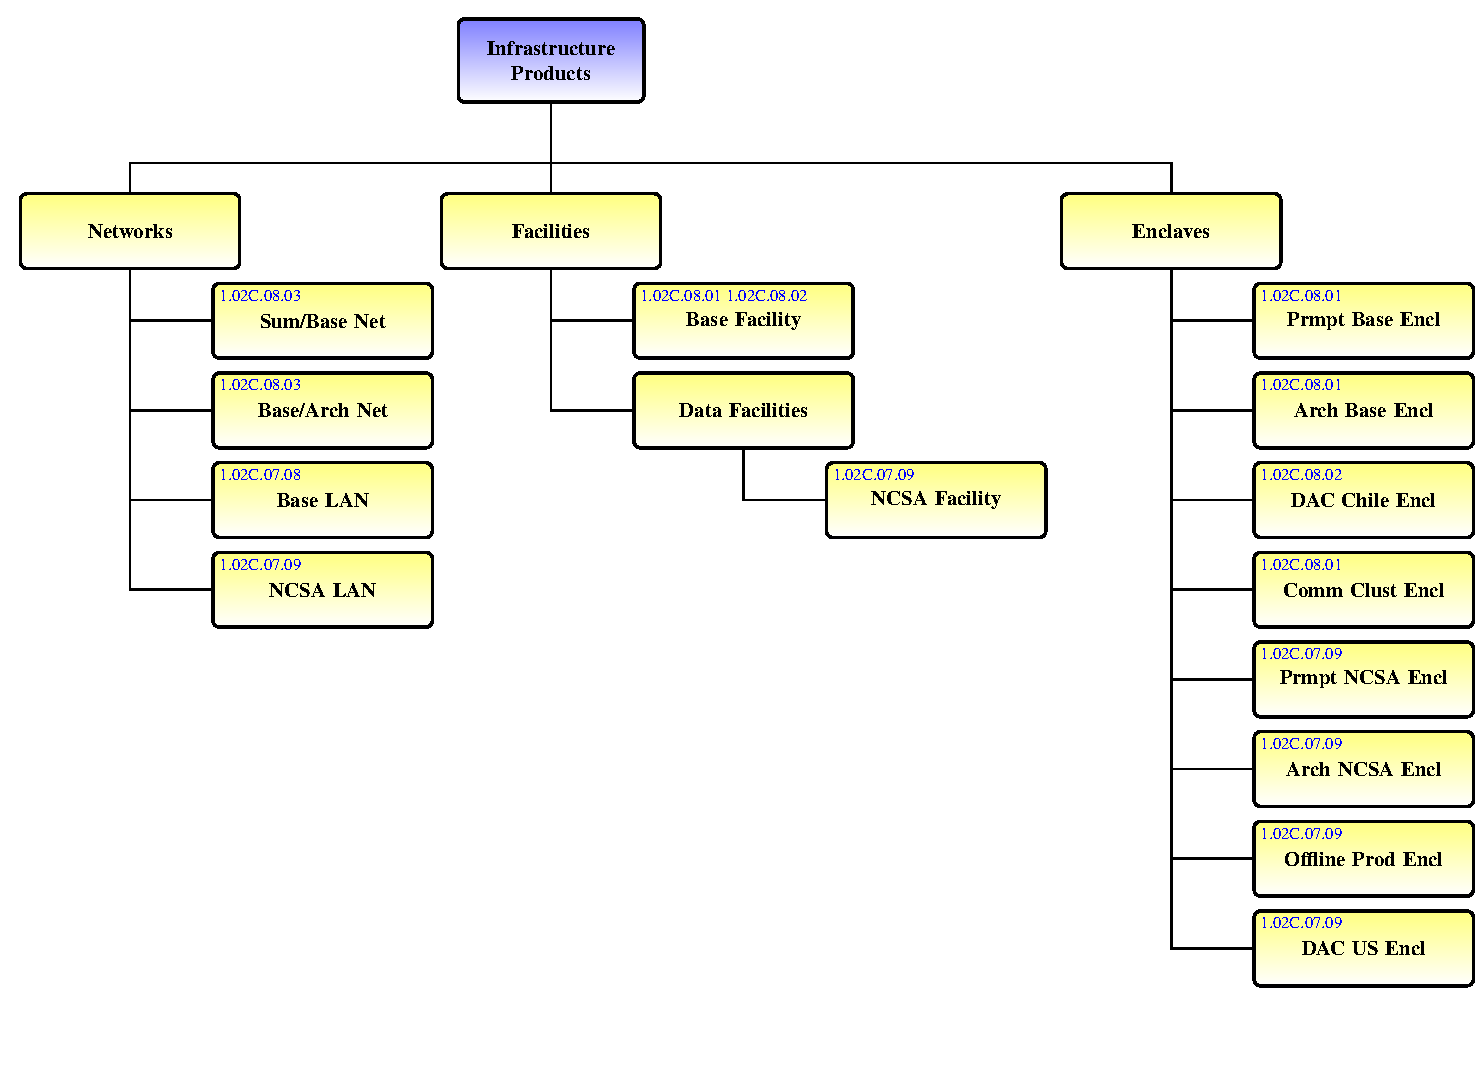
\includegraphics[width=0.9\textwidth]{figs/Main_INFRA}
	\end{center}
	\caption{Subset of the product tree from \citeds{DMTN-104} pertaining to Infrastructure \label{fig:prodinfra}}
\end{figure}

\subsubsection{Data transfer and preservation}
Within the services mentioned in \reqref{req:otherservs} there are a set of services concerning data
transfer, preservation and tracking. These bear particular scrutiny.

\reqsimp{}{}{}{}{}
{
 Prospective awardees shall transfer data from Chile. This data shall be archived, tracked and made
 available to Rubin processing systems.  See specifically \secref{sec:dbb}
}\\

Butler currently keeps track of files in Postgres and can be used with filesystems or S3.
S3 seems more scalable long term. See also \reqref{req:butler}

\reqsimp{}{}{}{}{}
{
 Image data shall be ingested into the Rubin butler. Files shall be accessible via an
 S3 compliant object store interface.
}\\

\reqsimp{}{}{}{}{}{}
{
	The facility  should provide a Postgres like database service for the Butler metadata.
	This service shall allow Rubin to  select extensions like PGSphere.
	It shall by performant for databases up to 100 TB.
	}

\reqsimp{}{}{}{}{}{}
{
	Any data services provided (filesystems, object stores, databases) shall be regularly backed up for disaster recovery, unless otherwise specified (e.g., /scratch).
}\\\\


These services are currently known  as Data backbone (DBB) - these could be installed/ported.




